\documentclass[border=5pt]{standalone}
\usepackage{graphicx}
\usepackage{xcolor}
\usepackage{tikz}
\usetikzlibrary{arrows.meta,calc}

\definecolor{flowBlue}{HTML}{2F6FED}
\definecolor{flowCyan}{HTML}{079C9A}
\definecolor{flowOrange}{HTML}{E98A00}
\definecolor{flowRed}{HTML}{D64545}
\definecolor{flowPurple}{HTML}{7040C8}
\definecolor{flowGreen}{HTML}{168B61}

\tikzset{
    module/.style={inner sep=0pt, outer sep=3pt},
    arrowbase/.style={-{Latex[length=2.5mm,width=1.8mm]}, line width=1.35pt,
        preaction={draw=white, line width=3.5pt}},
    obsblue/.style={arrowbase, draw=flowBlue},
    obscyan/.style={arrowbase, draw=flowCyan},
    actorflow/.style={arrowbase, draw=flowOrange},
    riskflow/.style={arrowbase, draw=flowRed},
    mapflow/.style={arrowbase, draw=flowPurple},
    executeflow/.style={arrowbase, draw=flowGreen},
    trainflow/.style={arrowbase, draw=flowBlue, densely dashed},
    rewardflow/.style={arrowbase, draw=flowOrange, densely dashed}
}

\begin{document}
\begin{tikzpicture}
    % User-arranged modules. Arrows are intentionally drawn after all nodes.
    \node[module] (lidar) at (1.35,4.05)
        {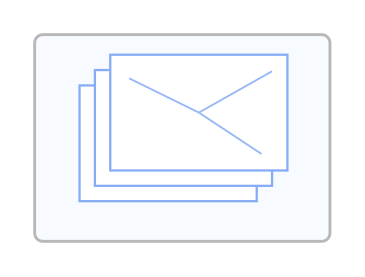
\includegraphics[width=2.25cm]{01_lidar_sequence.png}};
    \node[module] (lidarenc) at (4.10,4.05)
        {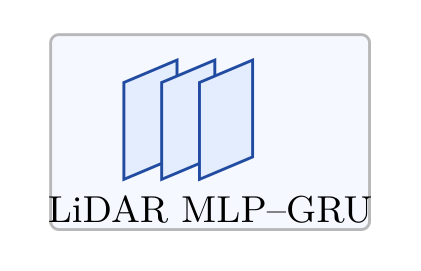
\includegraphics[width=2.35cm]{03_lidar_encoder.png}};
    \node[module] (state) at (1.35,1.45)
        {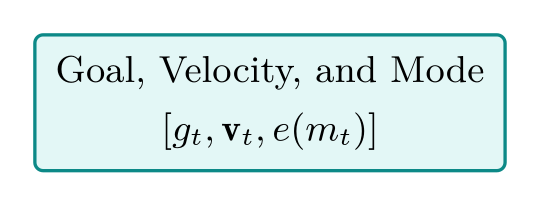
\includegraphics[width=2.50cm]{02_robot_state.png}};
    \node[module] (stateenc) at (4.10,1.45)
        {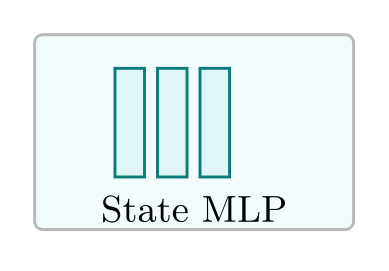
\includegraphics[width=2.25cm]{04_state_encoder.png}};
    \node[module] (fusion) at (6.15,2.72)
        {
\includegraphics[width=0.65cm]{05_fused_embedding.png}};

    \node[module] (actor) at (8.00,3.62)
        {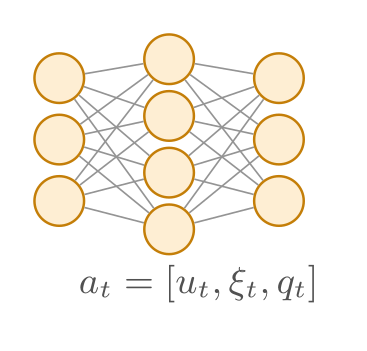
\includegraphics[width=1.90cm]{06_td3_actor.png}};
    \node[module] (pvo) at (10.10,3.62)
        {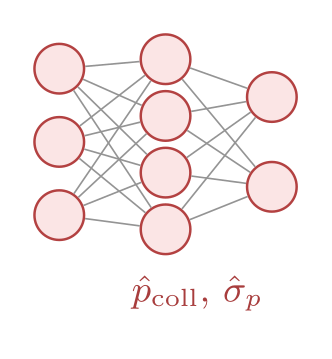
\includegraphics[width=1.72cm]{08_neural_pvo.png}};
    \node[module] (filter) at (12.10,3.72)
        {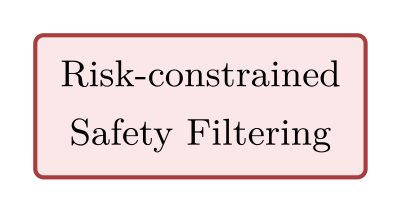
\includegraphics[width=1.55cm]{09_safety_filter.png}};
    \node[module] (mapper) at (14.15,3.72)
        {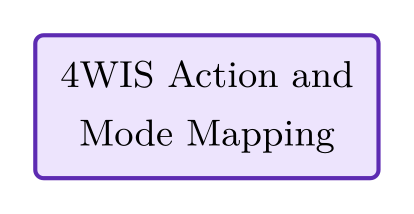
\includegraphics[width=1.58cm]{10_4wis_mapper.png}};
    \node[module] (velocity) at (16.35,3.72)
        {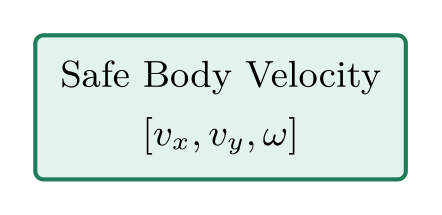
\includegraphics[width=1.72cm]{11_safe_velocity.png}};

    \node[module] (critic) at (8.00,1.25)
        {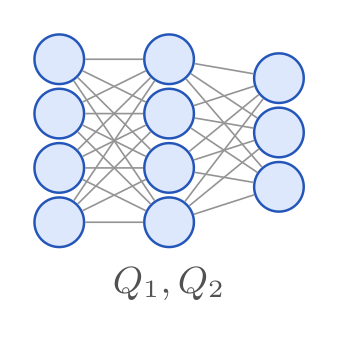
\includegraphics[width=1.78cm]{07_td3_critic.png}};
    \node[module] (irsim) at (10.55,1.25)
        {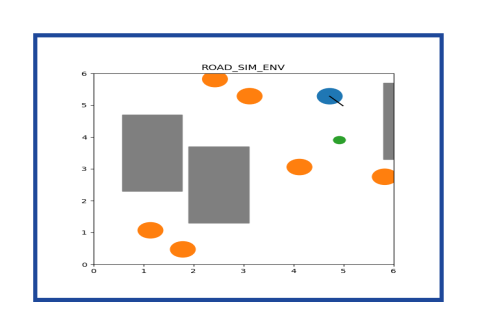
\includegraphics[width=2.32cm]{13_irsim_training.png}};
    \node[module] (reward) at (13.05,1.25)
        {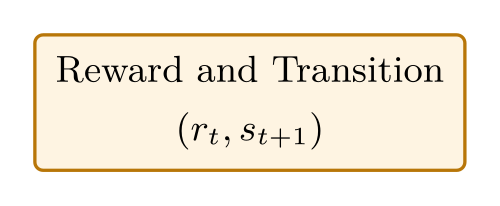
\includegraphics[width=1.80cm]{14_reward_transition.png}};
    \node[module] (gazebo) at (16.35,1.18)
        {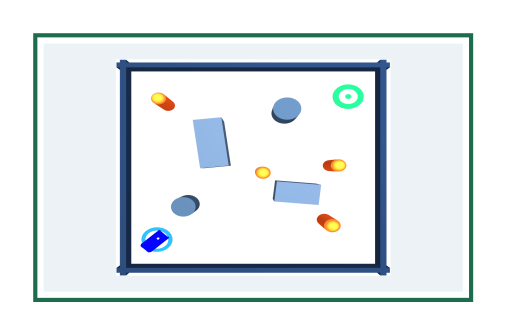
\includegraphics[width=2.52cm]{15_gazebo_validation.png}};

    % Observation branches and shared latent representation.
    \draw[obsblue] (lidar.east) -- (lidarenc.west);
    \draw[obscyan] (state.east) -- (stateenc.west);
    \draw[obsblue] (lidarenc.east) to[out=0,in=165] (fusion.north west);
    \draw[obscyan] (stateenc.east) to[out=0,in=195] (fusion.south west);

    % Shared features feed policy, critic, and the history-conditioned risk head.
    \draw[obscyan] (fusion.north east) to[out=20,in=180] (actor.west);
    \draw[obsblue] (fusion.south east) to[out=-20,in=180] (critic.west);
    \draw[obscyan] (fusion.north) to[out=78,in=135,looseness=1.15] (pvo.north);

    % Action-conditioned risk filtering and 4WIS execution.
    \draw[actorflow] (actor.east) -- (pvo.west);
    \draw[riskflow] (pvo.east) -- (filter.west);
    \draw[riskflow] (filter.east) -- (mapper.west);
    \draw[mapflow] (mapper.east) -- (velocity.west);
    \draw[executeflow] (velocity.south) -- (gazebo.north);

    % Training execution and Actor--Critic feedback.
    \draw[executeflow] (velocity.south west)
        to[out=-115,in=25,looseness=1.15] (irsim.north east);
    \draw[obsblue] (irsim.east) -- (reward.west);
    \draw[rewardflow] (reward.south)
        to[out=-90,in=-90,looseness=1.15] (critic.south);
    \draw[trainflow] (critic.north) -- (actor.south);
    \draw[actorflow, densely dashed] (actor.south east)
        to[out=-55,in=145,looseness=0.90] (irsim.north west);
\end{tikzpicture}
\end{document}
